\documentclass[
    12pt,
    a4paper,
    bibliography=totoc,
    cleardoublepage=em, 
    index=totoc,
    ngerman,
    openright,
    final,
    listof=nochaptergap,
]{scrbook}
\usepackage{scrhack}
\usepackage{cmap}
\usepackage[T1]{fontenc}
\usepackage[utf8]{inputenc}

% ##################################################
% Unterstuetzung fuer die deutsche Sprache
% ##################################################
%\usepackage{ngerman}
\usepackage[ngerman]{babel}
\usepackage{graphicx}
\usepackage{wrapfig}
\usepackage{lmodern}

% ##################################################
% Dokumentvariablen
% ##################################################

% Persoenliche Daten
\newcommand{\docNachname}{Mustermann}
\newcommand{\docVorname}{Max}
\newcommand{\docStrasse}{Straße}
\newcommand{\docOrt}{Ort}
\newcommand{\docPlz}{123456}
\newcommand{\docEmail}{student@hs-furtwangen.de}
\newcommand{\docMatrikelnummer}{000000}

% Dokumentdaten
\newcommand{\docTitle}{TITEL}
%\newcommand{\docUntertitle}{} % Kein Untertitel
\newcommand{\docUntertitle}{UNTERTITEL}
% Arten der Arbeit: Bachelorthesis, Masterthesis, Seminararbeit, Diplomarbeit
\newcommand{\docArtDerArbeit}{ART DER ARBEIT}
%Studiengaenge: Allgemeine Informatik Bachelor, Computer Networking Bachelor,
% Software-Produktmanagement Bachelor, Advanced Computer Scinece Master
\newcommand{\docStudiengang}{STUDIENGANG}
\newcommand{\docAbgabedatum}{11.11.2011}
\newcommand{\docErsterReferent}{ERSTER REFERENT}
%\newcommand{\docZweiterReferent}{-} % Wenn es nur einen Betreuer gibt
\newcommand{\docZweiterReferent}{ZWEITER REFERENT}

% ##################################################
% Allgemeine Pakete
% ##################################################

% Abbildungen einbinden
\usepackage{graphicx}

% Zusaetsliche Sonderzeichen
\usepackage{dingbat}

% Symbole Haken und X [OPTIONAL]
%\usepackage{pifont}
%\newcommand{\cmark}{\ding{51}}
%\newcommand{\xmark}{\ding{55}}

% Farben
\usepackage{color}
\usepackage[usenames,dvipsnames,svgnames,table]{xcolor}

% Maskierung von URLs und Dateipfaden
\usepackage[hyphens]{url}

% Deutsche Anfuehrungszeichen
\usepackage[babel, german=quotes]{csquotes}

% Pakte zur Index-Erstellung (Schlagwortverzeichnis)
\usepackage{index}
\makeindex

% Ipsum Lorem
% Paket wird nur für das Beispiel gebraucht und kann gelöscht werden
\usepackage{lipsum}

% ##################################################
% Seitenformatierung
% ##################################################
\usepackage[
	portrait,
	bindingoffset=1.5cm,
	inner=2.5cm,
	outer=2.5cm,
	top=3cm,
	bottom=2cm,
	%showframe, %Aktivieren um Seitengrenzen anzuzeigen
	%includeheadfoot
	]{geometry}

% ##################################################
% Kopf- und Fusszeile
% ##################################################

\usepackage{fancyhdr}

\pagestyle{fancy}
\fancyhf{}
\fancyhead[EL,OR]{\sffamily\thepage}
\fancyhead[ER,OL]{\sffamily\nouppercase{\leftmark}}

\fancypagestyle{headings}{}

\fancypagestyle{plain}{}

\fancypagestyle{empty}{
  \fancyhf{}
  \renewcommand{\headrulewidth}{0pt}
}

%Speichert \chaptermark in \oldchaptermark damit 
% es für die Anhänge zurückgesetzt werden kann
\let\oldchaptermark\chaptermark

%Kein "Kapitel # NAME" in der Kopfzeile
\renewcommand{\chaptermark}[1]{
	\markboth{#1}{}
   	\markboth{\thechapter.\ #1}{}
}

% ##################################################
% Schriften
% ##################################################

% Stdandardschrift festlegen
\renewcommand{\familydefault}{\sfdefault}

% Standard Zeilenabstand: 1,5 zeilig
\usepackage{setspace}
\onehalfspacing 

% Schriftgroessen festlegen
\addtokomafont{chapter}{\sffamily\large\bfseries} 
\addtokomafont{section}{\sffamily\normalsize\bfseries} 
\addtokomafont{subsection}{\sffamily\normalsize\mdseries} 
\addtokomafont{caption}{\sffamily\normalsize\mdseries} 

%Einrücken von Absätzen deaktivieren
\setlength{\parindent}{0pt}

%Zeilenabstand bei abstätzen
\usepackage{parskip}

% ##################################################
% Inhaltsverzeichnis / Allgemeine Verzeichniseinstellungen
% ##################################################

\usepackage{tocloft}

% Punkte auch bei Kapiteln
\renewcommand{\cftchapdotsep}{3}
\renewcommand{\cftdotsep}{3}

% Schriftart und -groesse im Inhaltsverzeichnis anpassen
\renewcommand{\cftchapfont}{\sffamily\normalsize}
\renewcommand{\cftsecfont}{\sffamily\normalsize}
\renewcommand{\cftsubsecfont}{\sffamily\normalsize}
\renewcommand{\cftchappagefont}{\sffamily\normalsize}
\renewcommand{\cftsecpagefont}{\sffamily\normalsize}
\renewcommand{\cftsubsecpagefont}{\sffamily\normalsize}

%Zeilenabstand in den Verzeichnissen einstellen
\setlength{\cftparskip}{.5\baselineskip}
\setlength{\cftbeforechapskip}{.1\baselineskip}

%Einrücken von Absätzen deaktivieren
%\setlength{\parindent}{0pt}

%Zeilenabstand bei abstätzen
\usepackage{parskip}

% ##################################################
% Abbildungsverzeichnis und Abbildungen
% ##################################################

\usepackage{caption}

\usepackage{wrapfig}

% Nummerierung von Abbildungen
\renewcommand{\thefigure}{\arabic{figure}}
\usepackage{chngcntr}
\counterwithout{figure}{chapter}

% Abbildungsverzeichnis anpassen
\renewcommand{\cftfigpresnum}{Abbildung }
\renewcommand{\cftfigaftersnum}{:}

% Breite des Nummerierungsbereiches [Abbildung 1:]
\newlength{\figureLength}
\settowidth{\figureLength}{\bfseries\cftfigpresnum\cftfigaftersnum}
\addtolength{\figureLength}{2mm} %extra offset
\setlength{\cftfignumwidth}{\figureLength}
\setlength{\cftfigindent}{0cm}

% Schriftart anpassen
\renewcommand\cftfigfont{\sffamily}
\renewcommand\cftfigpagefont{\sffamily}

%standardpfad anpassen
\graphicspath{ {../src/content/pictures/} }

% ##################################################
% Tabellenverzeichnis und Tabellen
% ##################################################

% Nummerierung von Tabellen
\renewcommand{\thetable}{\arabic{table}}
\counterwithout{table}{chapter}

% Tabellenverzeichnis anpassen
\renewcommand{\cfttabpresnum}{Tabelle }
\renewcommand{\cfttabaftersnum}{:}

% Breite des Nummerierungsbereiches [Abbildung 1:]
\newlength{\tableLength}
\settowidth{\tableLength}{\bfseries\cfttabpresnum\cfttabaftersnum}
\addtolength{\tableLength}{3mm} %extra offset
\setlength{\cfttabnumwidth}{\tableLength}
\setlength{\cfttabindent}{0cm}

%Schriftart anpassen
\renewcommand\cfttabfont{\sffamily}
\renewcommand\cfttabpagefont{\sffamily}

% Unterdrueckung von vertikalen Linien
\usepackage{booktabs}

%Multi row für spezifische zellen
\usepackage{multirow}

%Additional table package
\usepackage{tabu}

% ##################################################
% Listings (Quellcode)
% ##################################################

\usepackage{listings}

%use typewriter font which supports bold characters
\usepackage{beramono}

\definecolor{codegreen}{rgb}{0,0.6,0}
\definecolor{codegray}{rgb}{0.5,0.5,0.5}
\definecolor{codepurple}{rgb}{0.5,0,0.33}
\definecolor{codepurblue}{rgb}{0.16,0.0,1.0}
\definecolor{backcolour}{rgb}{0.95,0.95,0.92}

\lstdefinestyle{codestyle}{
    backgroundcolor=\color{backcolour},   
    commentstyle=\color{codegreen},
    keywordstyle=\bfseries\color{codepurple},
    numberstyle=\tiny\color{codegray},
    stringstyle=\color{codepurblue},
    basicstyle=\scriptsize\ttfamily,
    breakatwhitespace=false,         
    breaklines=true,                 
    captionpos=b,                    
    keepspaces=true,                 
    numbers=left,                     
    numbersep=5pt,                 
    showspaces=false,                
    showstringspaces=false,
    showtabs=false,                  
    tabsize=2
}

\lstset{style=codestyle}

%Code auschnitt importieren aus datei
%\mylisting{from}{to}{language}{file}{descr}{path}
\newcommand{\mylisting}[6]{
\lstinputlisting[language=#3,
				firstnumber=#1,
				firstline=#1,
				lastline=#2,
				caption={#4, #5}, 
				label={implementation_listing_#4_#5}]
				{#6}
}

% ##################################################
% Appendix
% ##################################################

%Calc packet für berechnungen
\usepackage{calc}

%Appendix paket, setzen der flags für das TOC
\usepackage[toc,title,titletoc]{appendix} 

%Umbenennen der überschrift für die Anhänge 
\renewcommand{\appendixtocname}{Anhänge}

%Befehl für einen neuen Bericht und die erste seite als bild
\newcommand{\appendixsection}[2]{
\section{#1}
\appendixsingle{#2}
}

%Befehl für einzelne seite als bild eingefasst, damit überschrift und kopfzeile
% bestehen bleibt. 
\newcommand{\appendixsingle}[1]{
\vspace{-10cm}
\vfill
\mbox{}\hspace{-1.5cm}\includegraphics[width=\linewidth+3cm]{#1}\hspace{-1.5cm}\mbox{}
\vspace{-10cm}
\vfill
\mbox{}
}

%Datenträger Tabelle
\definecolor{lightgray}{gray}{0.85}
\definecolor{ultralightgray}{gray}{0.95}
\definecolor{mygray}{gray}{0.70}

% ##################################################
% Theoreme
% ##################################################
  	
% Umgebung fuer Beispiele
\newtheorem{beispiel}{Beispiel}

% Umgebung fuer These
\newtheorem{these}{These}

% Umgebung fuer Definitionen
\newtheorem{definition}{Definition}
  	
% ##################################################
% Literaturverzeichnis
% ##################################################

\usepackage{bibgerm}

% ##################################################
% Abkuerzungsverzeichnis
% ##################################################

\usepackage[printonlyused]{acronym}

% ##################################################
% PDF / Dokumenteninternelinks
% ##################################################

\usepackage[
	colorlinks=false,
   	linkcolor=black,
   	citecolor=black,
  	filecolor=black,
	urlcolor=black,
    bookmarks=true,
    bookmarksopen=true,
    bookmarksopenlevel=3,
    bookmarksnumbered,
    plainpages=false,
    pdfpagelabels=true,
    hyperfootnotes,
    pdftitle ={\docTitle},
    pdfauthor={\docVorname~\docNachname},
    pdfcreator={\docVorname~\docNachname}]{hyperref}

% ####################################################
% Command für einfache QUellenangabe bei Bilder, etc.
% ####################################################

\newcommand{\source}[1]{\caption*{Quelle: {#1}} }


\begin{document}

\setcounter{secnumdepth}{3}

% Titelblatt
\begin{titlepage}
\pagestyle{empty}

% ##################################################
% HFU-Logo einbinden
% ##################################################
\begin{flushright}
\begin{figure}[ht]
\flushright

\includegraphics[height=3cm]{content/pictures/hfu.jpg}
\end{figure}
\end{flushright}

% ##################################################
% Titel
% ##################################################
\begin{center}
{\fontsize{18}{22} \selectfont \docArtDerArbeit}\\[5mm]
{\fontsize{18}{22} \selectfont im Studiengang} \\[5mm]
{\fontsize{18}{22} \selectfont \docStudiengang}\\
\vspace{1cm}
\begin{onehalfspace}
{\fontsize{22}{26} \selectfont \textbf{\docTitle}}\\[5mm]
{\fontsize{18}{22} \selectfont \docUntertitle}


\end{onehalfspace}
\end{center}

% ##################################################
% Zusatzinformationen
% ##################################################
\vfill
\begin{center}
\begin{tabular}{lcl}
Referent  		&:& \docErsterReferent 	\\ \\
Koreferent 		&:& \docZweiterReferent \\ \\	
Vorgelegt am 	&:& \docAbgabedatum 	\\ \\
Vorgelegt von 	&:& \docVorname~\docNachname\\
				& & Matrikelnummer: \docMatrikelnummer\\
				& & \docStrasse,~\docPlz~\docOrt	\\
				& & \docEmail			
\end{tabular}
\end{center}
\end{titlepage}
\cleardoubleemptypage

\frontmatter
\pagenumbering{Roman}

% Abstract
\chapter*{Abstract\markboth{Abstract}{}}
\addcontentsline{toc}{chapter}{Abstract}

[Englisches Abstract (100-120 Worte)]

[Deutsches Abstract (100-120 Worte)]
\cleardoubleemptypage

% Inhaltsverzeichnis
\phantomsection
\addcontentsline{toc}{chapter}{Inhaltsverzeichnis}
\tableofcontents
\cleardoubleemptypage

% Abbildungsverzeichnis einbinden und ins Inhaltsverzeichnis
% WORKAROUND: tocloft und KOMA funktionieren zusammen nicht
% korrekt\phantomsection
\phantomsection 
\addcontentsline{toc}{chapter}{\listfigurename} 
\listoffigures
\cleardoubleemptypage

% Tabellenverzeichnis einbinden und ins Inhaltsverzeichnis
% WORKAROUND: tocloft und KOMA funktionieren zusammen nicht
% korrekt\phantomsection
\phantomsection
\addcontentsline{toc}{chapter}{\listtablename}
\listoftables
\cleardoubleemptypage

%Define listing
\makeatletter
\begingroup\let\newcounter\@gobble\let\setcounter\@gobbletwo
  \globaldefs\@ne \let\c@loldepth\@ne
  \newlistof{listings}{lol}{\lstlistlistingname}
\endgroup
\let\l@lstlisting\l@listings
\makeatother
\setlength{\cftlistingsindent}{0em}
\renewcommand{\cftlistingsafterpnum}{\vskip0pt} %Spacing between entries
\renewcommand*{\cftlistingspresnum}{\lstlistingname~}
\settowidth{\cftlistingsnumwidth}{\cftlistingspresnum}


% Abkürzungsverzeichnis
\chapter*{Abkürzungsverzeichnis\markboth{Abkürzungsverzeichnis}{}}
\addcontentsline{toc}{chapter}{Abkürzungsverzeichnis}

\begin{acronym}
\acro{API}[API]{Application Programming Interface - Programmierschnittstelle}
\acro{BaFin}[BaFin]{Die Bundesanstalt für Finanzdienstleistungsaufsicht}
\acro{BAIT}[BAIT]{ Bankaufsichtliche Anforderungen an die IT}
\acro{BSI}[BSI]{Bundesamt für Sicherheit in der Informationstechnik}
\acro{DSGVO}[DSGVO]{Datenschutz-Grundverordnung}
\acro{ECM}[ECM]{Enterprise-Content-Management}
\acro{EDV}[EDV]{Elektronische Datenverarbeitung}
\acro{EU-GMP}[EU-GMP]{European Good Manufacturing Practice - Leitfaden der Guten Herstellungspraxis}
\acro{GPM}[GPM]{Geschäftsprozessmanagement}
\acro{GoBD}[GoBD]{Grundsätze zur ordnungsmäßigen Führung und Aufbewahrung von Büchern, Aufzeichnungen und Unterlagen in elektronischer Form, sowie zum Datenzugriff}
\acro{HFU}[HFU]{Hochschule Furtwangen University}
\acro{IT}[IT]{Informationstechnik}
\acro{KAIT}[KAIT]{Kapitalverwaltungsaufsichtliche Anforderungen an die IT}
\acro{QES}[QES]{Qualifizierte elektronische Signatur}
\acro{REST}[REST]{Representational State Transfer - Programmierparadigma für verteilte APIs, z.B. in Web-Services}
\acro{RSA}[RSA]{kryptographisches Verfahren nach  Rivest, Shamir und Adleman}
\acro{SHA}[SHA]{Secure Hash Algorithm}
\acro{TR-ESOR}[TR-ESOR]{Richtlinie: BSI-TR-03125}
\acro{VAIT}[VAIT]{Versicherungsaufsichtliche Anforderungen an die IT}
\end{acronym}

\mainmatter

\chapter{Einleitung}

Diese Thesis wurde mit Unterstützung der Firma levigo erstellt. Das im Rahmen der Thesis entstandene Softwaremodul kommt in einer neuen Softwarelösung zum Einsatz, die sich zum Zeitpunkt dieser Arbeit in Entwicklung befindet (Stand 08/2019).

\section{Die Unternehmensgruppe levigo}
Die levigo Gruppe ist eine auf \acs{IT}-Dienstleistungen und Software-Komponenten für das \acs{ECM}-Umfeld spezialisierte Unternehmensgruppe. Sie wurde 2001 bei einem Zusammenschluss von BMS (Bill Mair Software) und cogito Informationssysteme GmbH gegründet. Cogito war ebenfalls eine Unternehmensgruppe, die 1997, aus dem Zusammenschluss von Procon Systems GbR und cogito Gesellschaft für Elektronikentwicklung mbH, gegründet wurde.\\
levigo beschäftigt rund 80 Mitarbeiter und besitzt neben dem Hauptstandort Holzgerlingen noch zwei weitere Betriebstätten in Backnang. Die Firma ist Mitglied des Softwarezentrums Böblingen / Sindelfingen.\\
Die Unternehmensgruppe levigo teilt sich in drei Firmen auf: levigo holding ist das Dachunternehmen der Gruppe und übernimmt die Administration der Tochterunternehmen. Ihr Zuständigkeitsbereich sind alle Personalangelegenheiten, Fragen des Rechts, Controlling und Finanzen. Des Weiteren kümmert sich levigo holding um die Infrastruktur und Betriebsmittel der anderen Firmen.\\
levigo systems ist spezialisiert auf Client-Server-Anwendungen mit Virtualisierung, Storage und kontinuierlicher Verfügbarkeit. Sie bieten Komplettlösungen für Hardware-Konzeption und \acs{IT} Ausstattung aus einer Hand. Der Aufbau und die Optimierung von Firmennetzwerken und der \acs{IT}-Infrastruktur mittelständischer Unternehmen, ist die Kernkompetenz der Firma. Zusätzlich werden Dienstleistungen im Bereich \acs{IT}-Sicherheit angeboten. Angebotene Cloud-Dienste werden auf eigenen Servern in Süddeutschland betrieben.\\
levigo solutions bietet mit den jadice Softwareprodukten integrationsfreundliche und flexible Java-Komponenten für das \acs{ECM}-Umfeld an. Die Produkte ermöglichen plattformunabhängige Verarbeitung und Anzeige aller gängigen Archivierungs- und Officeformate. Zudem bietet levigo solutions mit den jadice Komponenten Lösungen für Kundenportale, Postkorblösungen, Rechercheclients und Datenmigrationsprozesse. Mit der neuen Produktlinie neverpile werden Teilgebiete des Geschäftsprozessmanagement (\acs{GPM}) abgedeckt.\cite{1}

\section{neverpile eureka}
Im Rahmen dieser Thesis wird ein Audit-Log-System implementiert und diskutiert. Das Audit-Log-System wird in "`neverpile eureka"' integriert.\\
neverpile eureka ist ein schlankes Enterprise Content Management System zur (Langzeit-) Archivierung von Dokumenten und anderen geschäftsrelevanten Artefakten. Die Software folgt dem "`\acs{API}-first-Prinzip"' und beschränkt sich auf wesentliche Kernfunktionalitäten. Alle weitergehenden kundenspezifischen Funktionen können modular ergänzt werden. Die modulare Struktur erlaubt eine einfache Integrierbarkeit in bestehende Systeme und Anbindung an beliebige externe Ressourcen. Auch sollen im Rahmen von neverpile eureka keine bereits gelösten Teilprobleme neu implementiert werden. Bereits existierende Lösungen für Teilprobleme werden eingebunden, nicht ersetzt. Die Software ist ein auf Container- und Clusterumgebung ausgelegtes System, welches dynamisch skalierbar und damit flexibel an Anforderungen angepasst werden kann. 
Zu den Spezifikationen von neverpile eureka gehört auch die Auditierung von Dokumenten. Diese wird im Rahmen dieser Thesis entworfen und implementiert.

\section{Audit-Logs}
Unternehmen und größere Organisationen führen Audit-Logs, um Ereignisse in ihren Informationssystemen langfristig festzuhalten. So gespeicherte Informationen dienen der Nachvollziehbarkeit interner Prozesse und ermöglichen deren Überwachung. Neben unternehmensinterner Prozesskontrolle und Auditierungsvorgaben kommen in vielen Geschäftsbereichen gesetzliche Vorgaben und Regelungen hinzu. Speziell die gesetzlichen Vorgaben verpflichten Unternehmen, Auskunft über verschiedene Informationen geben zu können\cite{8280477}. \\
Audit-Logs können beliebige Arten von Ereignissen dokumentieren. In dieser Thesis wird die Auditierung von Dokumentendaten in Langzeit-Archivsystemen betrachtet. Es soll ermöglicht werden, den kompletten Lebenszyklus sensibler Daten zu rekonstruieren. Alle Änderungen an einem Dokument werden zusammen mit Informationen zu den verantwortlichen oder beteiligten Akteuren festgehalten. Der Auditierungsvorgang prüft dann die Konsistenz und Authentizität der protokollierten Events.\\
Ein Audit-Log besteht aus uniformen Audit-Events, die eine inhärente Ordnung benötigen. Audit-Events können unterschiedliche Informationen enthalten und individuell an die jeweiligen Anforderungen angepasst werden. Die Anforderungen ergeben sich aus dem angestrebten Auditierungsprozess. Der Auditierungsprozess beschreibt den eigentlichen Nutzen des Audit-Logs. In diesem wird das Audit-Log ausgewertet und Informationen aggregiert oder gefiltert, um allgemeine Aussagen über Prozesse des Systems zu erhalten.\cite{7118074} Einträge in Audit-Logs müssen aussagekräftig genug sein, um alle Anforderungen einer späteren Auditierung zu erfüllen. Dem entgegen steht das Prinzip der Datensparsamkeit, die besagt, dass nur die notwendigsten Informationen dauerhaft gespeichert werden sollen.\cite{2458973}\\
Im Falle der Auditierung von Geschäftsdokumenten enthält ein Eintrag Informationen über die Akteure, die an dem Event beteiligt sind. Dabei ist insbesondere die eindeutige Identität des ausführenden Benutzers wichtig. Auch das tatsächliche Subjekt des Events, das betroffene Dokument, muss eindeutig identifizierbar sein. Die Art der Datenmanipulation und gegebenenfalls der Inhalt der Änderung muss ebenfalls festgehalten werden. Durch Festhalten des Zeitpunkts des Events, können alle Änderungen eines Dokuments in chronologische Reihenfolge gebracht werden. Interessant sind außerdem Kontextinformationen, wie die auslösende Schnittstelle und das Resultat des Events, das über Erfolg oder Fehlschlag informiert.\cite{7118074}\\
Über das Audit-Log kann somit jede Änderung der auslösenden Schnittstelle bzw. dem auslösenden Bearbeiter zugeordnet werden. So kann die Ursache für fehlerhafte oder manipulierte Dokumente nachvollzogen werden.\\
Unautorisierte Manipulationen können durch einen Abgleich des Ist-Zustands mit dem, im Audit-Log verifizierten, Soll-Zustands entdeckt werden. Da das Audit-Log so zu einer Validierungsinstanz wird, ist es ein potenzielles Ziel für Angriffe und Manipulation und muss entsprechend geschützt werden. Ein Angreifer kann durch Manipulation des Audit-Logs versuchen Änderungen oder Löschung von Dokumenten zu vertuschen oder falsche Schuldzuweisungen zu konstruieren. Besonders in Systemen, die ihre Datenspeicherung auslagern, z.B. in Cloud Storage Lösungen, ist es wichtig zu garantieren, dass die so bezogenen Daten nicht manipuliert wurden.\cite{6726483}\\
Um ads Audit-Log vor Manipulation zu schützen, gibt es verschiedene Herangehensweisen. In dieser Thesis wird eine Kombination digitaler Signaturen und manipulationssicheren Datenstrukturen betrachtet. Die digitalen Signaturen dienen dabei als vertrauenswürdige Ankerpunkte und die verwendete Datenstruktur soll vor Manipulationen interner und externer Quellen schützen.

\subsection{Audit-Log Anforderungen}
Die Anforderungen an das Audit-Log-System für neverpile eureka sind folgende:
\begin{itemize}
\item Erfassung aller relevanten Ereignisse von Dokumenten.\\
Die erfassten Daten enthalten: Zeitstempel, \acs{REST}-Schnittstellen URL, beteiligte Plugins (Facets), Änderungstyp, Ergebnis, Benutzerkennung, Dokumenten-Hash und Dokumenten-Id.
\item Audit-Log über alle Events.\\
Zusammenhängendes Audit-Log über alle modifizierenden Events aller Dokumente.
\item Audit-Log Events bezüglich eines einzeln Dokuments.\\
Zusammenhängendes Log mit allen modifizierenden Events eines einzelnen Dokuments.
\item Überprüfbarkeit der Integrität.\\
Die Integrität jedes Audit-Logs und jeder Teilausschnitt des Audit-Logs kann geprüft und bestätigt werden.
\item Verifikation eines Dokuments.\\
Der aktuelle Stand eines Dokuments muss über das Audit-Log verifiziert werden können.
\item Verifikation einzelner Audit-Events.\\
Jedes Audit-Event muss über seinen Inhalt verifizierbar sein.
\item Vollumfängliche Verifikation.\\
Ein effizientes Verfahren zur Verifikation aller Audit-Events wird benötigt.
\item Skalierbarkeit und synchronisierter Betrieb über mehrere neverpile Instanzen.\\
Der Betrieb über mehrere Container Instanzen muss ermöglicht werden und dynamisch skalierbar sein.
\item \acs{REST}-Schnittstelle.\\
Jede Funktion des Audit-Logs muss über eine \acs{REST}-Schnittstelle zugänglich sein.
\end{itemize}

\chapter{Grundlagen}

\section{Digitale Signaturen}
Digitale Signaturen sind vergleichbar mit einer handschriftlichen Unterschrift in digitaler Form. Die Signatur soll die Authentizität eines Datenobjekts beweisen, indem sie den genauen Inhalt unumstößlich mit einer Autorität verknüpft. Diese Autorität ist meist der Autor des Datenobjekts oder eine Instanz, die sich für den Inhalt verbürgt. Dabei muss sichergestellt sein, dass die Signatur nur mit einem geheimen Schlüssel, dem Private Key, erstellt werden kann. Dessen Inhalt darf nur dem Ersteller der Signatur bekannt sein. Die Signatur muss mit einem öffentlichen Schlüssel von jedem verifiziert werden können, dem Public Key. Das Ergebnis der Verifikation muss wiederum eindeutig dem Ersteller der Signatur zuzuordnen sein. Digitale Signaturen gehören somit zu den asymmetrischen kryptographischen Verfahren.\cite[S.29]{1841202}\cite[S.425f.]{548089}\\
Digitale Signaturen sind ein weit verbreitetes Verfahren in der Informationssicherheit und werden z.B. zur Authentifizierung, Daten-Integrität oder Nachweisbarkeit (Non-Repudiation) eingesetzt.\\
Grundlegende Definition\cite[S.426f.]{548089}:
\begin{enumerate}
\item Eine 'digitale Signatur' ist eine Datenfolge, welche ein digitales Datenobjekt mit einer Autorität assoziiert.
\item Ein 'Generierungsalgorithmus' erzeugt eine digitale Signatur.
\item Ein 'Verifikationsalgorithmus' für digitale Signaturen verifiziert die Authentizität der Signatur.
\item Ein 'Signaturschema' besteht aus einem Generierungsalgorithmus und den Verifikationsalgorithmen.
\item Ein 'digitaler Signierungsprozess' besteht aus einem Algorithmus zum Erstellen der Signatur und einer Konvertierung, welche Daten in ein signierbares Format überführt.
\item Der 'Verifikationsprozess' einer digitalen Signatur besteht aus einem Algorithmus zum Verifizieren einer Signatur und einer Konvertierung, welche Daten in ein verifizierbares Format überführt.\\
\end{enumerate}


\subsection{RSA}
\acs{RSA}, benannt nach den Entwicklern Ron Rivest, Adi Shamir und Leonard Adleman, ist das am weitesten verbreitete assymetrische Kryptosystem in der Informatik. \acs{RSA}  verwendet ein Schlüsselpaar, bestehend aus einem privaten Schlüssel, der zum Entschlüsseln oder Signieren verwendet wird, und einem öffentlichen Schlüssel, mit dem man Daten vertschlüsselt oder Signaturen prüft. Der private Schlüssel wird geheim gehalten und kann nicht aus dem öffentlichen Schlüssel berechnet werden. \acs{RSA} kann sowohl zum digitalen Signieren, als auch zum Verschlüsseln von Daten verwendet werden und benutzt eine sogenannte Einwegfunktion für die Verschlüsselung. Einwegfunktionen sind Funktionen, bei denen der Hinweg einfach zu berechnen ist, aber die Umkehrfunktion nur sehr schwer. \acs{RSA} nutzt dabei das mathematische Problem, dass es schwierig ist, die Faktorisierung großer Zahlen zu berechnen. Die Umkehrung ist jedoch trivial, da man beliebige, große Primzahlen multiplizieren kann, um eine große Zahl und ihre Faktorisierung zu erhalten. Um \acs{RSA} auch als Verschlüsselung benutzen zu können, muss die Einwegfunktion unter zuhilfenahme des Private Keys einfach zu berechnen sein. Mit dem öffentlichen Public Key kann eine mit dem Private Key erstellte Signatur validiert werden. Das \acs{RSA} Verfahren kann auch genutzt werden, um Daten mittels Public Key zu verschlüsseln. Diese können dann nur durch den zugehörigen Private Key wieder entschlüsselt werden. \cite[S.195, 200ff.]{1841202} \cite[S.433ff.]{548089}

\section{Hashfunktionen}
Eine Hashfunktion, im deutschen auch als Streuwertfunktion bezeichnet, ermöglicht es Daten beliebiger Größe auf Daten fester Größe abzubilden. Da diese Abbildungsfunktion typischerweise von einer größeren Wertemenge auf eine kleinere abbildet, kann es zu Kollisionen kommen. Daraus ergibt sich die Eigenschaft der Kollisionswahrscheinlichkeit der Hashfunktion. Eine gute Hashfunktion bildet möglichst selten unterschiedliche Eingabewerte auf denselben Hashwert ab. Hashfunktionen können auch speziell auf einen Typ von Eingangsdaten angepasst werden, um Kollisionen zu minimieren oder gar auszuschließen. Jedoch können allgemeine Hashfunktionen nie komplette Kollisionsfreiheit garantieren. Anwendungsbereiche für Hashfunktionen sind z.B. Schlüsselgenerierung von Hashtabellen, Passwortvalidierung, Prüfsummen und andere kryptographische Verifikationsverfahren.
Erstrebenswerte Eigenschaften von Hashfunktionen sind:
\begin{itemize}
\item Der komplette Abbildungsbereich soll unabhängig von der Eingabe gleichmäßig genutzt werden, um Kollisionen zu minimieren.
\item Ein minimal anderer Eingabewert eine genau so große Änderung am Ausgabewert bewirkt, wie jeder andere Eingabewert, dies wir als 'Chaos-' oder  'Lawineneffekt' bezeichnet.
\item Vom Ausgabewert sollen keine Rückschlüsse auf die Eingabe gemacht werden können. Weitergehend soll es auch keine Möglichkeit geben aus dem Ergebnis wieder den Ursprungswert zu berechnen.
\item Die Hashfunktion soll möglichst schnell berechenbar sein.
\end{itemize}
\cite[S.77ff.]{1841202}

\section{SHA-2}
\acs{SHA}-2 (Secure Hash Algorithm) ist eine Gruppe von Hashfunktion, die erstmals 2001 vom National Institute of Standards and Technology (NIST) standardisiert wurde. \acs{SHA}-2 ersetzt seinen Vorgänger \acs{SHA}-1 komplett, da dessen Sicherheit mittels einer Sicherheitslücke nicht mehr gewährleistet werden konnte. Mit \acs{SHA}-3 gibt es bereits seit 2015 einen Nachfolger zu \acs{SHA}-2. \acs{SHA}-3 verwendet ein Verfahren, das theoretische Schwächen von \acs{SHA}-2 eliminiert. Das neue Verfahren ist dadurch aber rechenintensiver. Da \acs{SHA}-2 bisher nicht gebrochen wurde, gibt es bisher keinen zwingenden Grund den neueren Algorithmus einzusetzen.
Die \acs{SHA}-2 Gruppe beinhaltet verschiedene Funktionen wie z.B. \acs{SHA}-256, \acs{SHA}-512, \acs{SHA}-512/256, \ldots Die Nummern am Ende stehen dabei für die verwendete Anzahl von Bits  und sind z.T. intern und extern verschieden. Bei einer Diskrepanz zwischen interner State-Größe in Bits und des zurückgegebenen Ergebnisses des Algorithmus wird im Namen erst die interne Anzahl an Bits, dann die Anzahl an Bits der Ausgabe angegeben. Die verschiedenen Funktionen wurden nach und nach in den Standard aufgenommen. Der neueste \acs{SHA}-2 Algorithmus wurde 2012 hinzugefügt.
Die vom NIST standardisierten Hashverfahren sind allgemein vertrauenswürdig und weit verbreitet. In Java und anderen Sprachen sind die \acs{SHA}-2 Algorithmen Teil der Standardbibliothek. \cite[S.82f]{1841202}

\section{Hashchains}
Eine Hashchain ist eine kryptographische Struktur, bei der aufeinanderfolgende Daten immer wieder mit in eine Hashfunktion verrechnet werden. Das Ergebnis der Hashfunktion ist der Element-Hash. Er wird in der Berechnung für das folgende Element mit einbezogen. So entsteht eine Kette von Hashwerten die rekursiv, aus dem jeweiligen Vorgänger Element-Hash und den Daten des zu verkettenden Elements berechnet werden. Der Element-Hash am Ende der Kette enthält somit die Verifikation über alle Elemente der Hashchain. Zur Verifikation kann die Berechnung ab einem beliebigen Punkt der Kette wiederholt werden. Wenn die erneut berechneten Hashwerte identisch zu den Originalen sind, ist garantiert, dass die verketteten Daten unverändert sind. Die Korrektheit dieser Verifikation basiert auf der Kollisionsresistenz der benutzten Hashfunktion.\cite[S.351ff]{40322788}

\section{Hashlists}
Hashlists ähneln Hashchains, jedoch sind die Elemente einer Hashlist unabhängig. Jedes Element einer Hashlist wird über eine Hashfunktion einem Hashwert zugewiesen. Die so generierten Einzel-Hashes werden wiederum zu einem Top-Hash zusammengefasst. Dieser Top-Hash verifiziert, wie schon bei der Hashchain, alle Daten in der Liste. Eine Verifikation ist aber durch Neuberechnung dieses Top-Hashes möglich. Es werden immer alle Hashwerte der Liste benötigt. Eine partielle Verifikation wie bei der Hashchain ist hier nicht möglich.\cite[S.18f]{326652}

\section{Merkle tree}
Der Merkle tree ist nach dem Erfinder Ralph Merkle benannt. Er wird auch als binärer Hashbaum bezeichnet. Merkle trees werden zum Zusammenfassen und der effizienten Integritätsüberprüfung großer Datensätzen verwendet. Bei Merkle trees werden die zu speichernden Daten und deren errechneter Hashwert in den Blättern abgelegt. Diese werden dann binärbaumtypisch in Paaren zu einem Elternknoten zusammengeführt. Der Elternknoten und alle weiteren Knoten bis zur Wurzel bilden ebenfalls einen Hashwert. Zur Berechnung dieser Hashes werden die bereits bekannten Hashwerte der Kind-Knoten zusammengefasst und erneut in die Hashfunktion eingegeben. Somit hält jeder Knoten mit seinem Hashwert eine prüfbare Verifikation der Integrität aller Knoten unter ihm. Im Falle eines Knotens mit nur einem Kind wird zur Berechnung des Eltern-Knotens der vorhandene Hash mit sich selbst konkateniert und wie gehabt verarbeitet. Dank der Baumstruktur kann in einem Merkle tree mit $N$ Elementen die Existenz eines gegebenen Elements mit einem Aufwand von $2 * log\textsubscript{2}(N)$ nachgewiesen werden, was ihn zu einer effizienten Datenstruktur macht.

\section{Blockchain}
Blockchain ist ein dezentrales System zum Speichern verifizierter Transaktionen. Einzelne Instanzen im Blockchain-Netzwerk werden als Nodes bezeichnet, diese arbeiten unabhängig und kontrollieren sich gegenseitig. Jeder Node hat die Möglichkeit neue Blöcke zu bilden oder Informationen aus den vorhandenen Daten abzurufen.\cite[S.197ff]{5841204}
\subsection{Blockchain-Datenstruktur}
Die Blockchain-Datenstruktur verbindet die oben genannten Verfahren und definiert ein Verfahrensprotokoll, um die Struktur zu verwalten. Die grundlegende Struktur einer Blockchain basiert auf einer normalen Hashchain. Jeder Block in der Kette verweist auf seinen Vorgänger. Zur Berechnung des Hashes eines neuen Blocks werden im Header Informationen aus dem Vorgänger mit einbezogen. Der Header besteht üb­li­cher­wei­se aus dem Hash des Vorgängers, dem Wurzel-Hash der Transaktions-Datenstruktur und Metainformationen für das Protokoll. Um die Transaktionsinformationen innerhalb eines Blocks abzubilden werden Merkle trees verwendet. \cite[S.197ff]{5841204}
\subsection{Blockchain-Forks}
Da Bockchain ein dezentrales System ist, kann es vorkommen, dass es temporär mehrere Kinder zu einem Block gibt. Das Hinzufügen eines neuen Blocks wird immer allen Teilnehmern des Systems mitgeteilt. Wenn jedoch zwei neue Blöcke zeitgleich entstehen, nennt man dieses Ereignis einen Blockchain-Fork. Dieser löst sich erst auf, wenn weitere Blöcke gefunden wurden. Teilnehmer der Blockchain arbeiteten immer an der Kette von Blöcken weiter, die am meisten Blöcke vom Ursprungsknoten entfernt ist. Wenn es nun konkurrierende Ketten gibt wird die Kette, die sich zuerst weiter vom Ursprungsknoten entfernt, durchsetzen. Im Falle eines so invalidierten Forks müssen alle dort eingetragenen Transaktionen auf einen Block in der aktuell gültigen Kette transferiert werden.\cite[S.199, 241ff]{5841204}
\subsection{Blockchain-Sicherheit}
Die Sicherheit einer Blockchain basiert auf der Abhängigkeit der Blöcke voneinander. Je älter ein Block in einer Blockchain ist, desto sicherer wird er. Zum Ändern eines Blocks ist eine komplette Neuberechnung aller Blöcke ab diesem Punkt nötig. Um einen Block anfügen zu dürfen, ist ein Konsensverfahren notwendig. Als solches wird beispielsweise eine "`Proof-Of-Work-Methode"' verwendet, welche Arbeit in der Form von Rechenleistung benötigt, um einen neuen Block zu "`finden"'. Der neue Block wurde unter Einsatz von viel Rechenleistung gesucht, die Validierung eines gefundenen Blocks ist wiederum einfach. Es kann aber auch eine beliebige andere Methode verwendet werden, um einen gemeinsamen Konsens zu erlangen. Wenn der Konsens gefunden wurde kann die Kette erweitert werden. Die Generierung eines Konsens soll dabei für eine einzelne Instanz schwierig sein um die Kontrolle zu dezentralisieren und Manipulationen zu vermeiden.\cite[S.219]{5841204}

\chapter{Gesetze und Richtlinien}
Die in dieser Arbeit beschriebene Audit-Log-Implementierung kann in verschiedenen Bereichen mit persönlichen Informationen angewandt werden. Insbesondere Daten im Medizin- und Finanzbereich unterliegen strengen rechtlichen Auflagen.\\
Da digitale Dokumente leicht manipuliert werden können, gibt es Gesetzte und Richtlinien, die die Prüfbarkeit der Echtheit digitaler Dokumente erfordern. Zusätzlich müssen Zugriffe beschränkt und dokumentiert werden. Gesetze und Richtlinien, die im Bezug auf das Audit-Log angewandt werden können, werden in diesem Kapitel erläutert. \cite{1966944}

\section{Nationales Recht}
Das Handelsgesetzbuch schreibt den Nachweis über Handelsbücher, Inventare, Eröffnungsbilanzen, Jahresabschlüsse, Einzelabschlüsse, Handelsbriefe und Belege für Buchungen vor. Die Nachweispflicht erlischt nach sechs oder zehn Jahren, je nach Dokumententyp.\cite{11}\\
Das Umsatzsteuergesetz schreibt das Aufbewahren von ausgestellten Rechnungen für mindestens zwei Jahre vor.\cite{12}\\
Die Abgabenordnung schreibt die Aufbewahrung aller steuerrelevanten Dokumente und deren Nachweis vor. Die Nachweispflicht erlöscht nach sechs oder zehn Jahren, je nach Dokumententyp.\cite{13}\\
Die Grundsätze zur ordnungsmäßigen Führung und Aufbewahrung von Büchern, Aufzeichnungen und Unterlagen in elektronischer Form, sowie zum Datenzugriff (\acs{GoBD}), ist eine Ergänzung zur Abgabenordnung und schreibt ebenfalls die Aufbewahrung steuerrelevanter Dokumente vor. Zusätzlich werden  Grundbucheinträge und allgemeine Geschäftsvorfälle eingeschlossen. Diese, 2014 erlassene, Verordnung ist im Vergleich mit der Abgabenordnung recht aktuell und geht explizit auch auf elektronische Datenverwaltung ein. Es werden Anforderungen an den Datenzugriff und die dauerhafte Verfügbarkeit gestellt. Die Anforderungen an die \acs{EDV} sind aber trotzdem sehr vage formuliert. Beispielsweise schreibt § 3.1 des \acs{GoBD} "`[...]angewandte Buchführungs- oder Aufzeichnungsverfahren müssen nachvollziehbar sein."'\cite{141} kein explizites Verfahren vor.\cite{14}

\section{Europa Recht}
Die europäische Datenschutz-Grundverordnung (\acs{DSGVO}) schreibt sowohl die Aufbewahrung bestimmter Dokumente, als auch deren Löschung vor. Die Aufbewahrung personenbezogener Daten wird mit sogenannten "`Löschfristen"' limitiert. Oft sind die Löschfristen mit der verpflichteten Aufbewahrungszeit gleichzusetzen.\cite{15}\\

\section{Richtlinien}

Der \acs{EU-GMP}(European Good Manufacturing Practice) Leitfaden schreibt zu computergestützten Systemen die Erstellung und die Auditierung von Audit-Logs expliziert vor, formuliert aber keine technischen Vorgaben.\cite{20} Die Richtlinie wurde in Deutschland 2003 in die Arzneimittel- und Wirkstoffherstellungsverordnung des  Bundesministerium für Gesundheit mit aufgenommen. \cite{19}\\

Die Bundesanstalt für Finanzdienstleistungsaufsicht (\acs{BaFin}) veröffentlichte im September 2018 die Kapitalverwaltungsaufsichtliche Anforderungen an die IT (\acs{KAIT}). Analog zur \acs{KAIT} veröffentlichte die \acs{BaFin} im September 2018 die Bankaufsichtliche Anforderungen an die IT (\acs{BAIT}) und im Oktober 2018 die Versicherungsaufsichtliche Anforderungen an die IT (\acs{VAIT}).\\
In diesen wird speziell auf den Umgang und die Verwaltung von Daten in den jeweiligen Unternehmensbereichen eingegangen, ohne jedoch konkrete Vorschläge von Verfahren zu definieren. Oft werden Anforderungen mit 
"`[\ldots] den Stand der Technik berücksichtigende Informationssicherheitsrichtlinien und Informationssicherheitsprozesse [\ldots]"' \cite{161} umschrieben. Es werden jedoch kryptographische Maßnahmen zum Schutz und zur Verifikation von Daten in \acs{IT} Systemen verlangt. Zudem wird eine Authentisierung und Protokollierung gefordert.\cite{16}\cite{17}\cite{18}

\subsection{TR-ESOR}
Das Bundesamt für Sicherheit in der Informationstechnik (\acs{BSI}) veröffentlichte die Publikation "`\acs{BSI} TR-03125 Beweiswerterhaltung kryptographisch signierter Dokumente"' kurz \acs{TR-ESOR}. Diese soll als Leitfaden gesehen werden und gibt präzise Vorschläge für Verschlüsselungs- und Signierung-Verfahren für Dokumente vor. Auch für die Architektur der Anwendung werden Vorgaben formuliert. Datenübertragung, Schnittstellen und Protokolle sind ausformuliert. Diese Richtlinie befindet sich zur Zeit dieser Arbeit noch in Entwicklung. \\
\acs{TR-ESOR} schlägt eine Dreiteilung der Sicherheitsstruktur vor. Die drei Teile bestehen aus einem \acs{API}-Modul, welches die Anwendung von den \acs{ECM}/Langzeitspeichersystemen abstrahiert. Ein Kryptomodul welches Funktionen für die Erstellung und Prüfung kryptographischer Sicherungsmittel bereitstellt. Zuletzt ein Signierungsmodul, welches als Bindeglied zwischen dem Kryptomodul, dem \acs{API}-Modul und dem \acs{ECM} dient. Hier werden die Kryptographischen Funktionen auf die zu verwaltenden Daten angewandt und entsprechend der \acs{API} weitergeleitet und verarbeitet.\\
Der Anwendungsbereich von \acs{TR-ESOR} beschreibt genau die Software die Gegenstand der Thesis ist. Die in dieser Arbeit vorgelegte Audit-Log-Implementierung hat sich an die Vorgaben von \acs{TR-ESOR} gehalten. Einzelne Vorgaben die den Rahmen dieser Thesis überschritten hätten wurden so behandelt, dass entsprechende Mechanismen später problemlos integriert werden können.\\
\acs{TR-ESOR} schlägt die Nutzung qualifizierter elektronischer Signaturen (\acs{QES}) vor. Die \acs{QES} kann von europäisch lizenzierten Verifikationsquellen erstellt werden und gilt somit als vertrauenswürdig. Die Benutzung solcher Signaturen ist nicht Gegenstand dieser Thesis, jedoch ist deren Nutzung und Einsatz für die Zukunft geplant. Gleiches gilt für die Nutzung von e-Cards. e-Cards sind physikalische und verifizierte Karten mit denen vertrauenswürdige benutzerauthentisierte Signaturen erstellt werden können. \cite{2}

\chapter{Vulnerabilität}
In größeren Softwaresystemen ist das Auditsystem nur eine Teilkomponente des Geasmtsystems. Im Betrieb wird über Schnittstellen mit zum Teil externen Datenquellen und anderen Akteuren kommuniziert. Aber nicht alle diese Akteure sind uneingeschränkt vertrauenswürdig. Um dennoch mit diesen arbeiten zu können, benötigt man Kontrollmechanismen, um externe Daten validieren zu können.\cite{8494085}\\
Eine Bedrohung bzw. Verwundbarkeit der Softwarekomponente kann entweder von außen, durch öffentliche Schnittstellen, oder von innen, mit Zugriff auf Systeminformationen wie  private Schlüssel, erfolgen.\cite{8574150}

\section{Angriffe von Außen}
Das verwendete Speichermedium ist ein großer Risikofaktor, da dieses Daten unabhängig verwaltet. Es muss sichergestellt sein, das abgelegte Daten unverändert wieder abgerufen werden können. Wenn ein Angreifer Zugriff auf das externe Speichermedium erlangt, könnte dieser Daten nach Belieben manipulieren. Auch unbeabsichtigte Manipulation durch Datenkorruption ist eine Gefahr. Das Schützen des Speichermediums vor unbefugten Manipulationen ist schwierig und nicht Teil dieser Arbeit. Es können aber Verfahren eingesetzt werden, die nach dem Abruf von Daten, deren unveränderten Zustand validieren kann. Die Validierung kann mithilfe digitaler Signaturen oder anderer asynchroner kryptographischer Verfahren garantiert werden. Digitale Signaturen können von vertrauenswürdigen externen Quellen generiert und validiert werden und somit den Inhalt der Daten validieren.\\
Der zweite Risikofaktor ist jeder reguläre Akteur oder Nutzer des Systems. Aktionen, die durch offizielle Schnittstellen zur Verfügung gestellt werden, müssen mithilfe von Nutzungsbeschränkungen geschützt werden. Alle Akteure, die ein Audit-Event auslösen, müssen sich authentisieren. Authentisierung ist der eindeutige Nachweis, dass es sich um einen bekannten Akteur handelt. Zudem muss der Akteur autorisiert sein. Autorisierung beschreibt das Einräumen von speziellen Rechten zur Interaktion mit dem System. Nur ein bekannter und berechtigter Akteur darf ein Audit-Event auslösen.\\
Zusammenfassend kann man folgern, dass jede Interaktion mit einem nicht systemeigenen Akteur, nicht vertrauenswürdig ist und für jede bereitgestellte Funktionalität müssen entsprechende Kontrollmechanismen vor Missbrauch schützen. Auch jede vom System genutzte externe Ressource muss auf Integrität geprüft werden.\cite{8494085}

\section{Angriffe von Innen}
Selbst wenn Daten mittels digitaler Signaturen validiert sind, ist es immer noch möglich Daten zu fälschen bzw. zu manipulieren, wenn man Zugriff auf den Signierungsschlüssel hat. Im Fall des Audit-Logs bedeutet dies beispielsweise, dass ein Systemadministrator die Möglichkeit hat, unbemerkt Daten zu manipulieren. Das Verhindern von Manipulationen durch berechtigte Benutzer mit vollem Zugriff auf das System ist äußerst schwierig. Es gibt jedoch Mechanismen die Daten zu schützen, auch wenn ein Nutzer die Berechtigung hat Änderungen vorzunehmen. Ein solcher Mechanismus ist es eine Hashstruktur zu bilden, bei der jedes neue Element auf die Daten seiner Vorgänger verweist und somit jede Änderung an bestehenden Daten sofort zu einer Inkonsistenz in der Hashberechnung führt, die nachgewiesen werden kann. Je mehr Daten für die Hashberechnung einbezogen werden, desto sicherer wird es deren Integrität zu beweisen. Aber auch diese Maßnahme ist nicht unfehlbar, denn der Angreifer hat die Möglichkeit die gesamte Hashverifikation mit seinen manipulierten Daten neu zu berechnen. Dies bedeutet aber einen enormen Aufwand und erfordert beträchtliche Zeit und Rechen-Ressourcen und kann so wiederum bemerkt werden. Das System kann durch die inkrementelle Abhängigkeit der Daten keine neuen Daten verarbeiten bevor die Neuberechnung nicht abgeschlossen ist. \cite{8494085} \cite{8574150} \cite{3286985}

\chapter{Analyse}

\section{Manipulationssichere Datenstrukturen}
Wie im Kapitel Vulnerabilität beschrieben ist es schwierig, Manipulation von Daten durch autorisierte Benutzer zu verhindern. Jedoch ist es möglich Manipulationen zu entdecken. Damit diese Erkennung funktioniert, muss die Datenstruktur einige Mechanismen unterstützen: \\
Das Hinzufügen eines Eintrags $X\textsubscript{i}$ in die Datenstruktur erzeugt eine Verifikation $C\textsubscript{i}$.\\
$Add(X) {\rightarrow} C\textsubscript{i}$.\\
Aus dieser Verifikation kann ein inkrementeller Beweis angefertigt werden, der die direkte Nachbarschaft zweiter Elemente belegt \\
$VerInc(X\textsubscript{i}, C\textsubscript{i-1}) {\rightarrow} C\textsubscript{i}$. \\
Wenn es zwei Elemente $C\textsubscript{i}$ und $C\textsubscript{j}$ aus der Datenstruktur gibt, dann gibt es eine eindeutige Reihenfolge von $i > j$ oder $i < j$. In beiden Fällen kann ein transitiver Beweis erstellt werden, der belegt, dass es eine konsistente Verbindung zwischen den beiden Elementen gibt und somit die Konsistenz des Logs zwischen $i$ und $j$ belegt $VerMember(C\textsubscript{i}, C\textsubscript{j}) {\rightarrow} ({\top},{\perp})$. \\
Mit diesen Grundregeln kann bewiesen werden, dass ein Element zur Datenstruktur gehört und es kann ein beliebig großer Ausschnitt des Logs verifiziert werden. \cite{8280477}\\
\\
\subsection{Analyse Hashchains}
Wie in Kapitel Grundlagen beschrieben sind Hashchains eine in sich abgesicherte Datenstruktur.Durch ihre rekursive Erstellung ist diese gut für die Audit-Log-Führung geeignet. Elemente in einer Hashchain haben immer eine feste Reihenfolge. Die Konsistenz zwischen Elementen kann überprüft werden, da die Hashchain von jedem Punkt aus mit dem dortigen Hashwert und den darauffolgenden Elementen neu berechnet werden kann. Wenn nun das Ergebnis des neuberechneten Hashwertes vom erwarteten Hashwert abweicht, ist bewiesen, dass die Daten nicht in ihrem Ursprungszustand vorliegen. \\
Hashchains haben für das Einfügen von Elementen eine konstante Komplexität. Die benötigte Zeit beim Überprüfen von Elementen ist linear.\cite[S.351ff]{40322788} \\
\\
\subsection{Analyse Merkle tree}
Merkle trees erfüllen die Anforderungen ebenfalls. Durch ihre Baumstruktur erhalten sie den Zugriff auf alle Blätter in logarithmischer Zeit. Bei der Verwendung von Merkle trees gibt es aber einige Besonderheiten zu beachten.\\
Die größte Nachteil ist, dass sich beim Hinzufügen von Einträgen (Blättern) Einträge in der Datenstruktur ändern anstatt lediglich die neuen Daten anzuhängen. Es ändern sich je nach Baumgröße und momentanen Zustand interne Knoten. Dies erfordert eine erneute Berechnung aller Knoten ab der Änderung bis zur Wurzel, um die Integrität des Baumes wieder herzustellen. Dieses Verhalten hat zwei Probleme zur Folge: Wenn nur ein einzelner Wert (die Wurzel), wie bei statischen Daten, als Verifikation gespeichert wird, dann verliert diese bei jeder Änderung ihre Gültigkeit. Solange der Baum klein ist, ist der Aufwand zum Einfügen eines Knotens noch gering, jedoch steigt der Aufwand je größer der Baum wird. Um den Aufwand zum Einfügen der Knoten zu verringern kann man den Baum so anlegen, dass alle Blätter des Baumes dieselbe Tiefe besitzen. Wenn der Baum voll ist, wird der Baum nicht neu ausbalanciert, sondern es wird über der Wurzel ein neuer Knoten eingesetzt. Der daraus resultierende Baum hat damit die Kapazität für doppelt so viele Blätter. Dieses Vorgehen hat den Vorteil, dass möglichst viele Knoten im Baum so früh wie möglich einen finalen Wert und feste Position beziehen. So können Beweise abgespeichert werden, die maximal einen Knoten pro Ebene des Baumes beinhalten. Ein Knoten des Baumes, der sich nicht mehr ändert, beweist die Konsistenz aller Knoten und Blätter unter sich. \\
Ein weiterer Nachteil ist, dass zum Erweitern der Bäume nicht nur ein simpler Top-Hash nötig ist, sondern eine beliebig große Menge von Daten kann Einfluss auf neu eingefügte Elemente haben. Dies kann bei beliebig großen Bäumen und begrenztem Arbeitsspeicher problematisch werden. Die Menge an Informationen die aus einem Baum minimal benötigt wird kann durch einen Algorithmus zur Findung von minimalen Verifikation eines Baumzustands erlangt werden.\cite{8280477} \cite{8280476}\\ 
\clearpage
Der Einfügeprozess anhand eines Beispiels: \\
Im Folgenden betrachten wir das beispielhafte Erweitern eines Merkle trees von der initialen Größe von sechs Knoten um jeweils einen Knoten in vier Schritten. Dabei erhalten wir einen Einblick in die Best- und Worst-Case Szenarien. Für die Legende der Abblidungen siehe Tabelle \ref{tab:TreeProofTable1}.

\begin{table}[!htb]
\caption{Legende: Einfügeoperation}
\label{tab:TreeProofTable1}
\begin{tabular}{|l|l|}
\hline
\textbf{Knoten} & \textbf{Beschreibung}
\\ \hline
Grün & \begin{tabular}[x]{@{}l@{}}Kleinste Menge an Knoten für einen Beweis für den neu eingefügten\\
Knoten. Diese Knoten sind bereits stabil und werden sich durch weitere \\
Einfüge-Operationen nicht mehr ändern.\end{tabular}
\\ \hline
Orange & \begin{tabular}[x]{@{}l@{}}Diese Knoten sind instabil und werden sich beim Erweitern des Baumes\\
noch ändern.\end{tabular}
\\ \hline
Blau & \begin{tabular}[x]{@{}l@{}}Stabile Knoten, die nicht zum Beweis gehören. Deren Hashwert wurde\\
bereits für die Erstellung der aktuell grünen Knoten verwendet\\
und diese konnten somit vernachlässigt werden.\end{tabular}
\\ \hline
Weiß & \begin{tabular}[x]{@{}l@{}}Weiße Knoten sind Platzhalter für später einzufügende Knoten. Diese\\
Knoten entstehen nur als rechter Knoten zu einem einzelnen Knoten\\
ohne Partner, damit der Baum bis zur Wurzel berechnet werden kann.\\
Der Hashwert dieser Knoten entspricht dem seines Nachbarns.\end{tabular}
\\ \hline
\end{tabular}
\end{table}

\begin{figure}[!htb]
	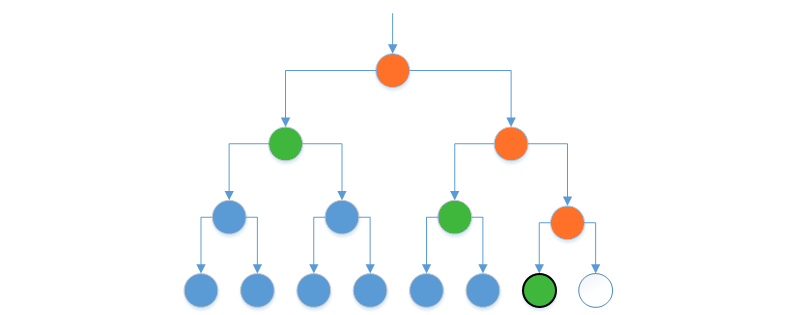
\includegraphics[width=1\textwidth]{content/pictures/TreeProof1}
	\caption{Schritt 1: einfügen Knoten 7}
	\label{fig:TreeProof1}
\end{figure}

In Schritt eins (siehe Abbildung \ref{fig:TreeProof1}) wird der siebte Knoten eingefügt. Als Beweis werden das Blatt selbst, und ein Knoten aus jeder Ebene außer der Wurzel gespeichert. Dies ist der Worst-Case da dies die maximal benötigte Anzahl an Knoten für diese Baumgröße ist. Der weiße Platzhalter-Knoten wird benötigt um den Baum bis zur Wurzel berechnen zu können und stellt darüber hinaus sicher, dass in allen höheren Ebenen Änderungen auftreten sobald der Platzhalter duch einen normalen Knoten ersetzt wird. Somit ist auch die Stabilität des Baums der Worst-Case, da in jeder Ebene außer den Blättern ein instabiler Knoten existiert.\\
\begin{figure}[!htb]
	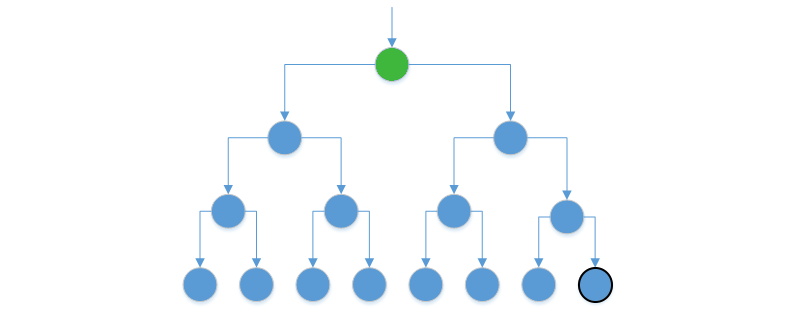
\includegraphics[width=1\textwidth]{content/pictures/TreeProof2}
	\caption{Schritt 2: einfügen Knoten 8}
	\label{fig:TreeProof2}
\end{figure}
\\
Im Gegensatz dazu ist Schritt zwei (siehe Abbildung \ref{fig:TreeProof2}) ein Best-Case. Der Baum ist voll und daher ist nun die Wurzel stabil und kann als Beweis für alle Unterknoten verwendet werden. Außerdem ist der Baum komplett stabil und es existieren keine instabilen Knoten.\\
\begin{figure}[!htb]
	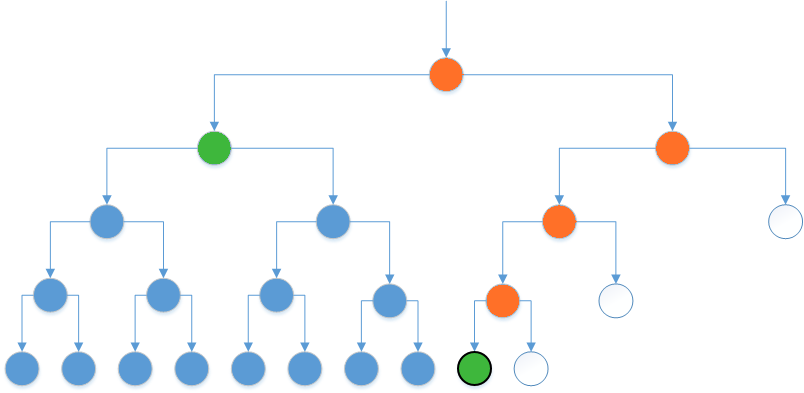
\includegraphics[width=1\textwidth]{content/pictures/TreeProof3}
	\caption{Schritt 3: einfügen Knoten 9}
	\label{fig:TreeProof3}
\end{figure}
\\
In Schritt drei (siehe Abbildung \ref{fig:TreeProof3}) muss der Baum, um den neunten Knoten einzufügen, erweitert werden. Da der Baum nicht neu balanciert wird, bleibt der alte Unterbaum stabil und es werden für jede Baumebene außer der Wurzel, temporäre Knoten verwendet, um den nächsten Knoten einzufügen. Der Beweis für diese Baumkonfiguration besetht aus der letzten Probe und dem neuen Knoten. Die Stabilität ist erneut ein Worst-Case, da es maximal viele instabile Knoten gibt.\\
\begin{figure}[!htb]
	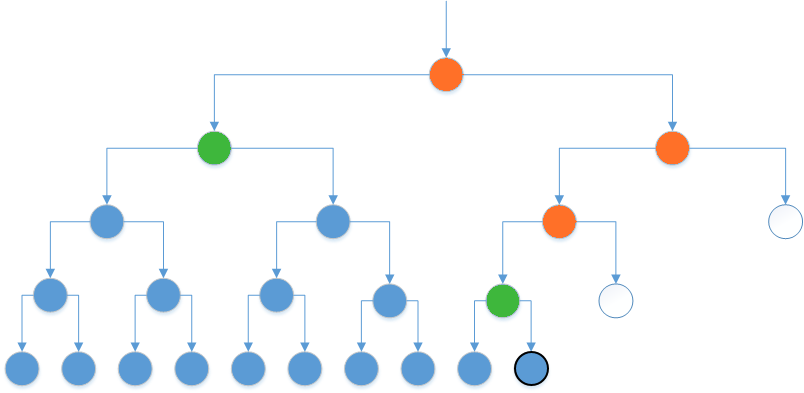
\includegraphics[width=1\textwidth]{content/pictures/TreeProof4}
	\caption{Schritt 4: einfügen Knoten 10}
	\label{fig:TreeProof4}
\end{figure}
\\
Zuletzt wird in Schritt vier (siehe Abbildung \ref{fig:TreeProof4}) der zehnte Knoten eingefügt, welcher bereits einen stabilen Knoten im neuen Unterbaum erzeugt. Die Menge an temporären und instabilen Knoten wurde jeweils um eins reduziert.\\

Zum Beweisen der Nachbarschaft zweier Knoten kann analog zu einer normalen Hashchain aus dem Beweis der Konsistenz des Vorgängerknoten und dem aktuellen Knoten der Beweis des Knotens rekonstruiert werden. Ist der Knoten unverändert, wird dies durch ein identisches Ergebnis bestätigt.\\

Um Knoten acht zu überprüfen (siehe Abbildung \ref{fig:TreeProof5} und Tabelle \ref{tab:TreeProofTable2}) wird der Beweis von Knoten sieben (in Gelb dargestellt) und der zu überprüfende Knoten selbst (in lila) gebraucht. Wenn nun der grüne Beweisknoten durch erneuerte Berechnung auf Basis des Beweises seines Vorgängers errechnet werden kann, ist die Konsistenz bewiesen.
\clearpage 
\begin{table}[!htb]
\caption{Legende: Beweiskonstruktion}
\label{tab:TreeProofTable2}
\begin{tabular}{|l|l|}
\hline
\textbf{Knoten} & \textbf{Beschreibung}
\\ \hline
Lila & \begin{tabular}[x]{@{}l@{}}Zu prüfender Knoten\end{tabular}
\\ \hline
Gelb & \begin{tabular}[x]{@{}l@{}}Beweis für den Vorgängerknoten des zu prüfenden Knotens.\end{tabular}
\\ \hline
Grün & \begin{tabular}[x]{@{}l@{}}Beweis des zu prüfenden Knotens.\end{tabular}
\\ \hline
Orange & \begin{tabular}[x]{@{}l@{}}Knoten, die für die Rekonstruktion des grünen Beweises erneut\\
berechnet werden müssen.\end{tabular}
\\ \hline
Blau & \begin{tabular}[x]{@{}l@{}}Für diesen Fall irrelevante Knoten.\end{tabular}
\\ \hline
Weiß & \begin{tabular}[x]{@{}l@{}}Platzhalter Knoten für diesen Fall irrelevant.\end{tabular}
\\ \hline
\end{tabular}
\end{table}

\begin{figure}[!htb]
	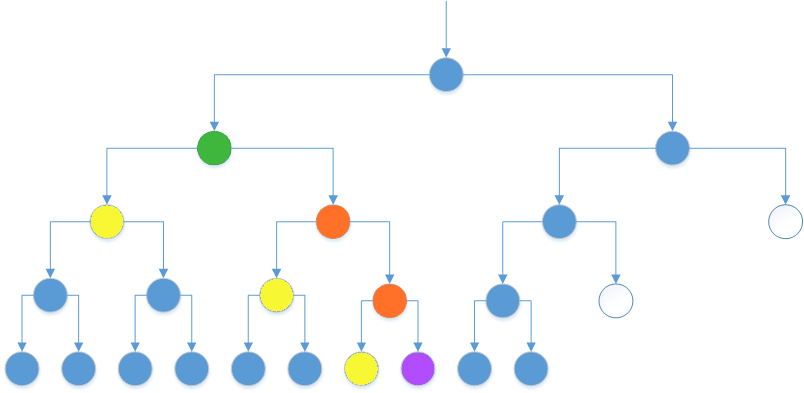
\includegraphics[width=1\textwidth]{content/pictures/TreeProof5}
	\caption{Beweis für Blatt 8}
	\label{fig:TreeProof5}
\end{figure}

Durch dieses Verfahren kann nun eine Validierung und Einfüge-Operationen in den Baum mit minimalen Informationen über den Baum realisiert werden und es müssen nicht alle Informationen über den kompletten Baum geladen werden. 

\section{Das "`Total Ordering"' Problem}
Das Total Ordering Problem beschreibt den Sachverhalt, dass in verteilten Systemen nicht immer klar festgestellt werden kann, in welcher exakten Reihenfolge Ereignisse eingetreten sind. Durch parallele Prozesse können Elemente zeitgleich bearbeitet werden. Erschwerend dazu kommt, dass die Kommunikation zwischen den Instanzen unzuverlässig und latenzbehaftet ist. In vielen Anwendungsfällen muss jedoch eine feste Reihenfolge bestimmt werden. Dies ist z.B. beim Erfassen von Systemübergreifenden Audit-Logs der Fall.\cite{359563}\\
Um diesem Problem zu begegnen, können verschiedene Mechanismen verwendet werden. Der trivialste Fall sind hochauflösende Zeitstempel. die Grundidee eines hochauflösenden Zeitstempels besagt, dass die Auflösing immer so hoch gewählt werden kann, dass zwischen beliebigen zwei Ereignissen eine zeitliche Differenz besteht. Die offensichtliche Problematik bei diesem Verfahren ist, dass es unabhängig von der Präzision des Zeitstempels, theoretisch immer trotzdem zu Kollisionen kommen kann. In verteilten Systemen gibt es außerdem ein grundsätzliches Problem: Alle Instanzen nutzen ihre eigenen Systemuhren. Um die Uhren zu synchronisieren kann ein entsprechendes Protokoll zwischen den Instanzen geschaffen werden. Hierbei ist die Herausforderung, dass die Kommunikation zwischen Instanzen latenzbehaftet ist. Latenzzeiten müssen bei der Synchronisation mit in Betracht gezogen werden. Dabei entstehen besonders dann Fehler, wenn die Latenz fluktuiert.\cite{315340}\\
Wenn zu einer zeitlichen Synchronisation im Cluster ein Protokoll zur Kommunikation zwischen den Instanzen erforderlich ist, kann man dieses Protokoll auch auf den vorliegenden Anwendungsfall spezialisieren. In einem solchen Protokoll einigen sich die Instanzen des Clusters auf eine gemeinsame Reihenfolge ohne eine zeitliche Komponente zu verwenden. Es gibt unterschiedliche Protokolle, die eine einheitliche Reihenfolge im Cluster garantieren können. Dabei unterscheiden sich zwei grundsätzliche Ansätze.\\
Im ersten Ansatz wird eine autoritäre Instanz bestimmt, über die alle anderen Instanzen die Reihenfolge erfragen müssen. Da diese Instanz eigenständig über die Reihenfolge entscheidet, wird die Reihenfolge nach der deren Bearbeitungsreihenfolge bestimmt. So kann im einfachsten Fall eine inkrementelle Sequenznummer vergeben werden. Dieses Verfahren hat folgende Nachteile: Da die Reihenfolge aller Events vieler Instanzen über eine einzelne Instanz vergeben wird, kann diese zum Engpass werden und damit die Geschwindigkeit des Gesamtsystems beeinträchtigen. Insbesondere bei Ausfällen hat dies drastische Auswirkungen auf das Gesamtsystem. Ein Lösungsansatz im Störungsfall einer autoritären Instanz wäre z.B. eine neue Instanz von allen aktiven Teilnehmern des Clusters zu wählen. Diese übernimmt dann temporär oder permanent die Funktion der ausgefallenen Instanz.\cite{565838}\\
Ein anderer Ansatz eines solchen Protokolls ist der Einsatz von Broadcasts und Majority-Voting. Wenn eine Instanz ein neues Element in die Sequenz einfügen will, wird diese Anfrage allen anderen Instanzen mitgeteilt. Wenn nun über die Hälfte der Instanzen dieses Element als das unmittelbar nächste in der Sequenz bestätigen, kann sichergestellt werden, dass das Cluster sich auf diese Reihenfolge einigt. Wenn aber die Hälfte des Clusters die Anfrage verneint, muss für die Transaktion der aktuelle Listenkopf aktualisiert und die Anfrage wiederholt werden. Diese Verfahren verursacht eine größere Netzlast, da mehr Kommunikation zwischen den Instanzen stattfinden muss, jedoch ist die Fehler und Ausfalltoleranz durch die dezentrale Struktur deutlich verbessert.\cite{1041682}\\


\chapter{Architektur}

\section{Systemarchitektur}
neverpile eurekas Systemarchitektur legt den Fokus auf Modularität. Der Kern des Systems beschränkt sich auf die Basis-Funktionalität. Weitere Funktionalität soll in optionalen und austauschbaren Modulen implementiert werden. So konstruierte Softwaremodule werden fortfolgend Facets genannt. Facets in neverpile eureka haben die Möglichkeit strukturell vordefinierte \acs{REST}-Schnittstellen zu implementierten oder auf Lifecycle-Events von Dokumenten zu reagieren.\\
Für die Nutzung gemeinsamer Ressourcen, wie persistentem Speicher oder Indizierungssystemen, werden in Core Interfaces definiert. Diese Anbindungen werden wiederum modular von Facets implementiert und garantieren, dass neverpile eureka ohne harte Abhängigkeiten flexibel in jeder Umgebung eingesetzt werden kann. Die Komposition von Facets, die in einer Instanz von neverpile eureka gemeinsam genutzt werden sollen, können mittels Annotationen und Konfigurationsdateien bestimmt werden.\\
Ein solches Facet ist auch Inhalt dieser Thesis sein. Das Facet, soll für die Auditierung von Dokumenten verantwortlich sein. 

\begin{figure}[!htb]
	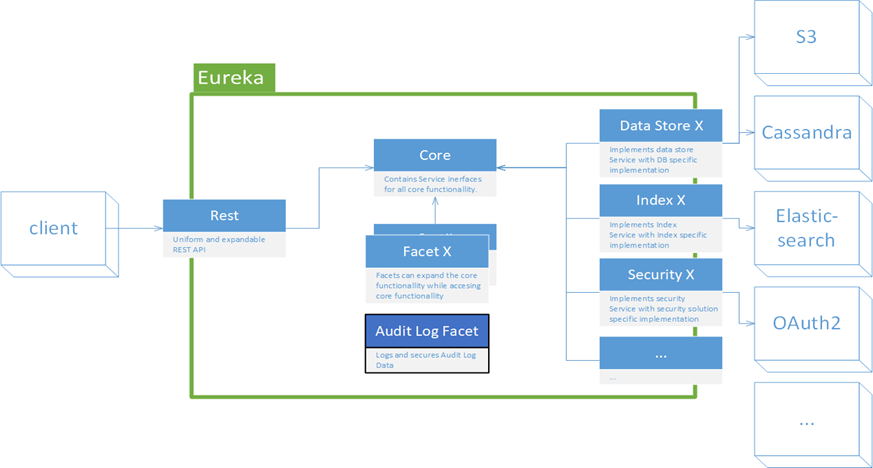
\includegraphics[width=1\textwidth]{content/pictures/eureka}
	\caption{Eureka System Überblick}
	\label{fig:eureka}
\end{figure}

Wie in Abbildung \ref{fig:eureka} dargestellt bietet eureka eine homogene \acs{REST}-Schnittstelle an, welche alle Funktionen zur Verfügung stellt. Eureka nutzt und aggregiert dabei eine Vielzahl bestehender Technologien. 

Das zu implementierende Audit-Facet nutzt dabei alle Möglichkeiten des Eureka Modells. Es werden eigene \acs{REST}-Endpunkte zur Durchführung von Audits angeboten. Das Facet reagiert auf Lifecycle-Events des Dokuments, die das Dokument verändern und nimmt diese Änderungen in das Audit-Log auf. Entsprechende Events sind die Erstellung, die Löschung und die Modifikation von Dokumenten. Über den Core angebotene Ressourcen wie persistenten Speicher und Synchronisationsmechanismen werden ebenfalls zur Erstellung des Audit-Logs verwendet.

\section{Datenmodell}

Für das Audit-Facet werden neue, mit den Dokumenten verknüpfte Daten gespeichert. Die Struktur dieser Daten ist flexibel und kann je nach Anforderung angepasst werden. Fester Bestandteil jeder Implementierung bleibt jedoch das Audit-Event selbst, als kleinste Kerneinheit. Jedes Audit-Log besteht aus vielen dieser Einheiten. Dort sind alle, für das Audit relevanten, Daten über ein einzelnes Ereignis gespeichert. Als eindeutige Identifizierung der Audit-Events wird eine Kombination aus der Dokumenten-ID und einem hochauflösenden Zeitstempel gewählt. Da die Dokumenten-ID einzigartig unter allen Dokumenten ist und jedes Dokument zu jedem Zeitpunkt nur von einem Event verändert werden kann, ist die so generierte ID kollisionsfrei und jedes Audit-Event kann eindeutig identifiziert werden. Auch die ID-Generierung ist modularisiert und kann durch alternative Implementierungen ersetzt werden.\\
Alle Audit-Logs sind fest einem Dokument zugeordnet. So kann ein Audit-Log über ein einzelnes Dokument bezogen werden. Die Beziehung zwischen Audit-Log und Dokument ist lediglich eine Referenz. Die eigentliche Datenstruktur, die alle Audit-Logs zusammenhält, überspannt alle Events.\\
Um Audit-Events zu schützen wird eine Sicherheitsschicht über jedes Audit-Event gelegt. Diese soll garantieren, dass der Inhalt der Events unverändert und konsistent mit allen anderen Events ist. Die genaue Implementierung der Sicherheitsschicht kann mit verschiedenen kryptographischen Strukturen implementiert werden und ist abermals modular und austauschbar.\\
Um eine übermäßig große Anzahl resultierender Audit-Dateien zu vermeiden, werden Audit-Logs in zeitlich abgegrenzte Blöcke aggregiert. Die Referenz von Dokument zu Audit-Event verweist also nicht direkt auf das jeweilige Event, sondern auf den Block, in dem das Event gespeichert ist. Diese Blockstruktur beschleunigt zusätzlich die Verifikation, da so die Anzahl der Speicherzugriffe reduziert wird.

\section{Service Architektur}


\begin{figure}[!htb]
	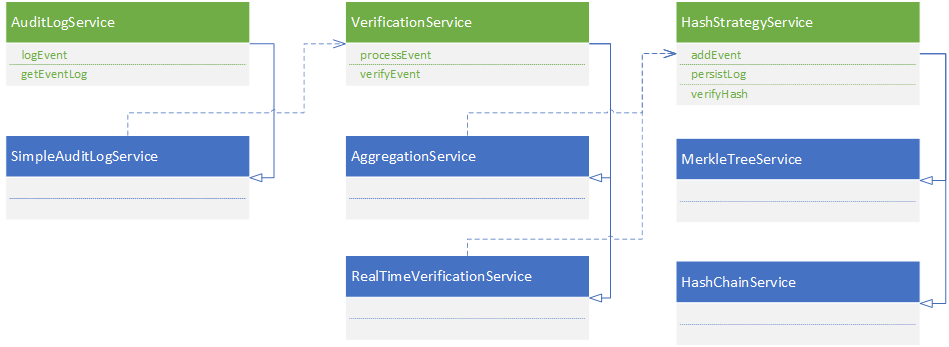
\includegraphics[width=1\textwidth]{content/pictures/services}
	\caption{Service Architektur}
	\label{fig:Services}
\end{figure}

Die Service Architektur des Audit-Log-Facets besteht aus drei Interfaces \label{fig:Services} und deren Implementierungen. 

\subsection{Audit-Log-Service}
Der Audit-Log-Service ist die Schnittstelle zur restlichen Anwendung. Hier werden alle Auslöser für neue Events gesammelt und verarbeitet. Lifecycle-Events werden hier verarbeitet und entsprechende Audit-Events generiert. Die Audit-Events lösen im Allgemeinen das Erstellen eines neuen Eintrags im Audit-Log aus. Auch die \acs{REST}-Ressourcen kommunizieren direkt mit diesem Service. Ein Auditor kann, auf diesem Weg, Verifikationsanfragen für Dokumente, einzelne Events oder das gesamte Log stellen. 

\subsubsection{Implementierung}
Die Lifecycle-Events von Dateien, für die ein Audit-Log erstellt werden soll, können in einer Konfiguration festgelegt werden. Die entsprechenden Events werden anhand dieser Konfiguration gefiltert und verarbeitet. Der Audit-Eintrag wird an den Object Store übergeben, um dieses zu mit Bezug auf den aktuellen Block zu persistieren. Zugleich wird der das Event an den Verification-Service übergeben, um die entsprechende Verifikation zu erstellen. Direkte Anfragen über die Audit-Log-REST-Schnittstelle werden in gleicher Weise an den Objektstore oder den Verification-Service weitergeleitet.

\subsection{Verification-Service}
Der Verification-Service wird vom Audit-Log-Service benutzt und ist sowohl für die Erstellung von Verifikationen als auch für die Verifikation selbst verantwortlich. Des Weiteren wird hier die Verarbeitungsstrategie festgelegt. Die Verarbeitungsstrategie umfasst die Art der Validierung, das Erstellen von Signaturen und die Aggregation von Events. 

\subsubsection{Implementierung}
Für den Verification-Service wurden zwei verschiedene Implementierungen erstellt. Eine erste, simple Implementierung erstellt die Verifikation synchron in der Transaktion, die das Event erzeugt hat. Dieses Verfahren hat neben der Einfachheit den Vorteil, dass die Verifikation innerhalb der Transaktion, die das Event auslöst, erstellt wird. Im Falle eines unerwarteten Fehlers bei der Erstellung der Verifkation, kann so die komplette Transaktion noch unproblematisch abgebrochen oder zurückgerollt werden. Ein weiterer Vorteil ist, dass die Verifikation unmittelbar nach seinem auslösenden Event verfügbar ist.\\
Die alternative Implementierung ist eine Aggregierung von Events zu Blöcken, die dann in einer größeren Transaktion gemeinsam persistiert werden. Vorteil dieser Variante ist die niedrigere Ressourcenanforderung, was einen höheren Datendurchsatz ermöglicht. Da viele Datenhaltungssysteme nicht auf viele kleine Transaktionen optimiert sind, wird diese Variante ab einer bestimmten Last unumgänglich.

\subsection{Hash-Strategy-Service}
Der Hash-Strategy-Service wird vom Verification-Service genutzt. Er bildet ein Interface um die Implementierung der kryptographischen Datenstruktur, deren Erzeugung und Manipulation zu kapseln. Hier werden die Daten für die Sicherheitsschicht, abhängig von der Implementierung, erzeugt und persistiert.

\subsubsection{Implementierung}
Auch für den Hash-Strategy-Service wurden zwei alternative Implementierungen erstellt. Die Erste ist eine Hashchain, die mit einem "`SHA-256"' Algorithmus die Daten der Audit-Events verknüpft. Diese Struktur bietet Flexibilität und ist einfach zu erweitern. Um die Sicherheit der Struktur zu unterstützen und vertrauliche Ankerpunkte in die Kette einzubauen, wird nach konstant vielen Einträgen eine Signatur zum aktuellen Hashwert erstellt. Von diesen Ankerpunkten aus ist die Zugriffszeit maximal $n$, wobei $n$ der Abstand zwischen den Signaturen ist.\\
Die zweite Variante ist eine Kombination aus Merkle tree und Hashchain. Es werden Merkle trees mit fester Größe erstellt. Diese werden wiederum als Hashchain verbunden. Das Verfahren benötigt einen größeren Rechenaufwand zum Erstellen neuer Knoten. Allerdings bietet der Baum Vorteile in Form von Sicherheit durch die höhere Vernetzung der Hashwerte. Die Zugriffszeiten auf ein Log-Event (Blatt) sind binärbaumtypisch logarithmisch. Zudem wird, ähnlich wie bei Hashchains, nach Abschluss jedes Merkle trees eine digitale Signatur der Wurzel erstellt um so alle im Baum enthaltenen Events zusätzlich abzusichern.

\section{Datenfluss}

\begin{figure}[!hbt]
	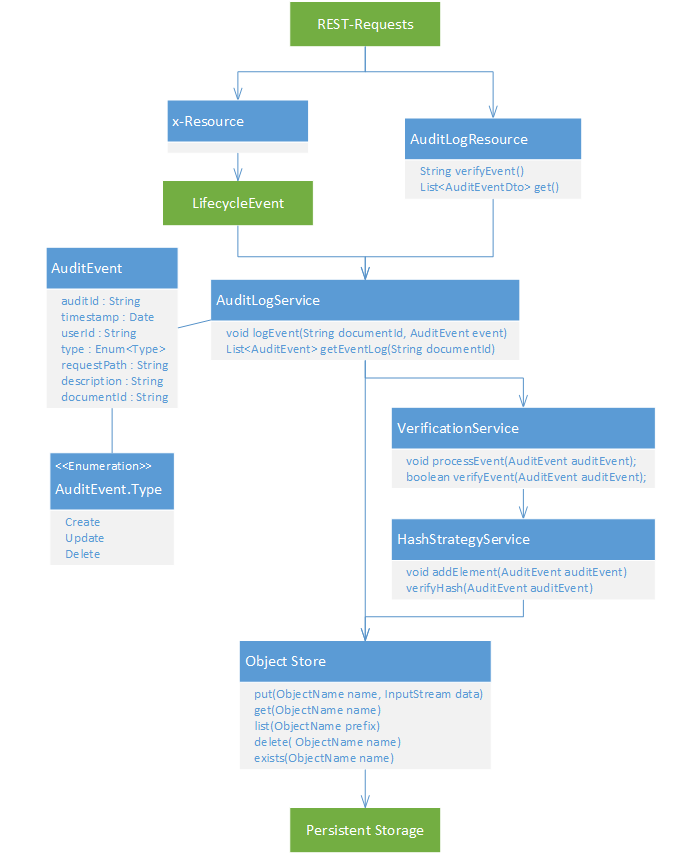
\includegraphics[width=1\textwidth]{content/pictures/auditflow}
	\caption{Anfragen-Fluss}
	\label{fig:auditflow}
\end{figure}

Der Datenfluss des Audit-Log-Facets ist in Abbildung \ref{fig:auditflow} dargestellt. Ausgehend von einer REST-Anfrage kann entweder direkt eine Ressource des Facets angesprochen werden oder eine andere Ressource löst ein relevantes Lifecycle-Event aus. Von diesem Punkt aus wird das Event, wie in der vorigen Sektion beschrieben, von den Audit-Services verarbeitet. Von den Services wird der Object Store genutzt um das Audit-Log selbst und die Verifikation zu persistieren oder bereits abgelegte Daten zu laden.

\section{Cluster-Scaling und Kommunikation}

\begin{figure}[!htb]
	\includegraphics[width=1\textwidth]{content/pictures/instances}
	\caption{Cluster Anfragen-Fluss}
	\label{fig:Instances}
\end{figure}

neverpile eureka ist darauf ausgelegt in einer Container-Umgebung ausgeführt zu werden. Alle Instanzen eines neverpile eureka Cluster sind gleichwertig. Die Instanzen haben alle einen identischen Umfang und Zuständigkeitsbereich. Es gibt keine Hierarchie und auch keine Abhängigkeiten zwischen Instanzen. Durch diese Homogenität ist ein On-Demand Scaling ein einfaches Zuschalten beliebig vieler weiterer Instanzen. Jede Anfrage an die \acs{API} wird von einem Loadbalancer entgegengenommen und dann an eine beliebige Instanz weitergeleitet (siehe Abbildung \ref{fig:Instances}). Die Kommunikation zwischen Instanzen ist minimal, wodurch diese unabhängig voneinander Anfragen bearbeiten können. Dieses Clustersystem erlaubt einfache Skalierung bei steigenden Anforderungen.

\section{Distributed processing}
Auch wenn die Instanzen von neverpile eureka so unabhängig voneinander arbeiten sollen wie es möglich ist, kommt man beim Thema Audit-logging nicht gänzlich um eine Synchronisation zwischen den Instanzen aus. Bei der Verifikation ist die Reihenfolge essenziell. Wenn mehrere Instanzen gleichzeitig Audit-Events auslösen, muss daher sichergestellt werden, in welcher globalen Reihenfolge die Events geordnet werden. Sich nur auf Timestamps zu verlassen ist in diesem Fall nicht ausreichend, da es zu identischen Timestamps kommen kann und die Synchronisation der lokalen Uhren der Instanzen nicht garantiert werden kann. Wenn also die rein zeitliche Bestimmung der Reihenfolge nicht zielführend ist, müssen komplexere Methoden verwendet werden. Die gewählte Lösung ist ein leichtgewichtiges Protokoll zwischen den Instanzen. Das Protokoll wird bereits an anderen Stellen in neverpile eureka verwendet und erzeugt deshalb keine zusätzlichen Abhängigkeiten. 
"`Distributed in Memory computing"' wird von vielen renommierten Frameworks benutzt und erlaubt es Daten zwischen Instanzen zu synchronisieren und atomare Operationen auf diesen auszuführen. Für die Implementierung der Lösung kann auf einige erprobte Open-Source-Lösungen, wie Apache Ignite oder Hazlecast, zurückgegriffen werden. Passend zum Gesamtkonzept von neverpile eureka werden keine Technologien vorgegeben. Es werden stattdessen Interfaces entwickelt, die mit einer frei gewählten Technologien implementiert werden können. Die einzige Anforderung des Audit-Logs, die Kommunikation zwischen den Instanzen erfordert, ist das Lösen des Total-Ordering-Problems. Dazu wird eine Distributed Atomic Reference verwendet. Diese Referenz wird zwischen allen Instanzen repliziert und der Zugriff reguliert. In dieser Referenz wird das neueste Event gespeichert. Die synchronisierte Referenz kann mit einer atomaren Funktion von jeder Instanz mit einem neuen Event aktualisiert werden. Durch die Referenz ist gewährleistet, dass alle Instanzen mit dem aktuellen Hash arbeiten und sich unmissverständlich auf eine Reihenfolge einigen.\cite{7496608}

\chapter{Ausblick} 
\chapter{Fazit}
Der Fokus der Thesis hat sich im Laufe der Analyse weg vom Blockchain-Ansatz, hin zu Hashchain-Technologien verschoben. Das Ziel der Thesis, ein durch Kryptographie abgesicherter Audit-Log zu entwerfen und zu implementieren, wurde dadurch nicht beeinflusst. Zu Beginn wurde Blockchain als technologische Grundlage gewählt. Die Analyse hat gezeigt, dass die inhärenten Vor- und Nachteil dieses Ansatzes nicht gänzlich auf die Anforderungen des Zielsystems neverpile eureka passen.\\
Da das Audit-Log-Facet nicht das Herzstück der Gesamtsoftware darstellt, diese aber um zusätzliche Funktionalität erweitert, sollte das Audit-Log so einfach wie möglich gehalten werden. Die vom Blockchain-Ansatz verwendeten "`Proof Of Work"'-Algorithmen, führen zu enormen Overhead und beeinflussen die Performance des Gesamtsystems negativ. Das simultane und somit redundante Arbeiten aller Nodes am selben Arbeitspaket erzeugt ebenso einen Overhead, der mit der in dieser Arbeit beschriebenen Lösung vermieden wurde. Die nötige Kommunikation zwischen einzelnen Instanzen ist, im Vergleich mit Blockchain, ebenfalls deutlich reduziert. Mit der Nutzung eines gemeinsamen Object Stores entfällt außerdem das Ablegen einer lokalen Kopie der Datenstruktur in jeder Instanz. Die Verwendung digitaler Signaturen als Ankerpunkt wird nur in der vorliegenden Lösung benötigt um Sicherheit zu gewärleisten. Bei Blockchain ist durch die starke Absicherung mittels Konsensalgorithmen keine weitere Absicherung notwendig.\\
Trotz dieser Unterschiede schützen beide Ansätze die Daten durch die inhärente Abhängigkeit in der verwendeten Datenstruktur. Dies führt in beiden Fällen dazu, dass jeder neue Eintrag in der Datenstruktur die Sicherheit der bereits vorhandenen Einträge erhöht.\\


% Schalgwortverzeichnis (Index)
%\printindex

% Literaturverzeichnis
\singlespacing
\bibliographystyle{alphadin}
\bibliography{bibtex}

% Eidesstattliche Erklärung
\chapter*{Eidesstattliche Erklärung\markboth{Eidesstattliche Erklärung}{}}
% Eintrag in das Inhaltsverzeichnis 
\addcontentsline{toc}{chapter}{Eidesstattliche Erklärung}

Ich versichere, dass ich die vorstehende Arbeit selbstständig verfasst und hierzu
keine anderen als die angegebenen Hilfsmittel verwendet habe. Alle Stellen der Arbeit die 
wörtlich oder sinngemäß aus fremden Quellen entnommen wurden, sind als solche kenntlich gemacht.
\\
\\
Die Arbeit wurde bisher in gleicher oder ähnlicher Form in keinem anderen
Studiengang als Prüfungsleistung vorgelegt oder an anderer Stelle
veröffentlicht.
\\
\\
Ich bin mir bewusst, dass eine falsche Erklärung rechtliche Folgen haben kann.

\vspace*{1.5cm} \par
\line(1,0){200} \par
\docOrt, \docAbgabedatum ~~\docVorname~\docNachname


%Zurücksetzen \chaptermark
\let\chaptermark\oldchaptermark

% Hier können Anhaenge angefuegt werden
\begin{appendices}
\chapter{Monatsberichte}
Nun folgen die Monatsberichte.
\newpage
\appendMultiPdfsection{Monatsbericht März}{content/attachments/Monatsbericht_Abschlussarbeit_1.pdf}
\appendMultiPdfsection{Monatsbericht April}{content/attachments/Monatsbericht_Abschlussarbeit_2.pdf}
\appendSinglePdfsection{Monatsbericht Mai}{content/attachments/Monatsbericht_Abschlussarbeit_3.pdf}
\appendSinglePdfsection{Monatsbericht Juni}{content/attachments/Monatsbericht_Abschlussarbeit_4.pdf}
\end{appendices}
\end{document}
